\section{Experiments}
\subsection{Data and Protocol}
We use 10{,}000 Grasp-Anything++ stems with one unique scene per stem and
split 8{,}000 train / 2{,}000 validation with seed 42, so the split is
scene-disjoint by construction.  All models train for 15 epochs, batch size 2,
learning rate $10^{-3}$, weight decay $10^{-4}$, and evaluation uses 10-step
respaced diffusion sampling.  A prediction is correct if it matches any
ground-truth rectangle with IoU $>0.25$ and angle error $<30^\circ$.

\begin{table}[t]
\centering
\caption{Repeated 10-step evaluation on 2{,}000 validation stems.  Final LSAR
uses scale $0.01$ and $\lambda_{\mathrm{aff}}=0.05$.}
\label{tab:main}
\footnotesize
\setlength{\tabcolsep}{3pt}
\begin{tabular}{lccc}
\toprule
Method & $\lambda_{\mathrm{aff}}$ & Correct & Mean\,$\pm$\,Std \\
\midrule
LGDM baseline & --- & 449 & $470.0\pm10.8$ \\
LSAR-no-aff & 0.0 & 643 & $653.7\pm6.5$ \\
LSAR-full & 0.1 & 625 & $605.3\pm18.9$ \\
LSAR (seed 42) & 0.05 & 686 & $\mathbf{678.0}\pm16.5$ \\
LSAR (seed 43) & 0.05 & 666 & $661.7\pm14.0$ \\
\bottomrule
\end{tabular}
\end{table}

\subsection{Results}
Table~\ref{tab:main} reports one training-loop evaluation and the mean over
three sampling evaluations.  The final method improves the baseline mean from
$470.0$ to $678.0$ (seed 42) and $661.7$ (seed 43).  Removing the auxiliary
affordance loss gives $653.7$; the larger weight $\lambda=0.1$ gives $605.3$.
LSAR therefore contributes mainly through spatial conditioning, while the
small affordance term is a useful auxiliary objective.  On a fixed
200-sample subset, 50 instead of 10 diffusion steps improves the baseline from
$39$ to $44$ correct and final LSAR from $65$ to $67$, preserving the ordering.

Figure~\ref{fig:qual} shows paired part-level examples.  The conditioned model
correctly locates a highlighter and keychain keys where the baseline fails and
retains success on an apple-stem case.  This illustrates that the refinement
improves spatial grounding rather than only global image semantics.

\begin{figure}[t]
\centering
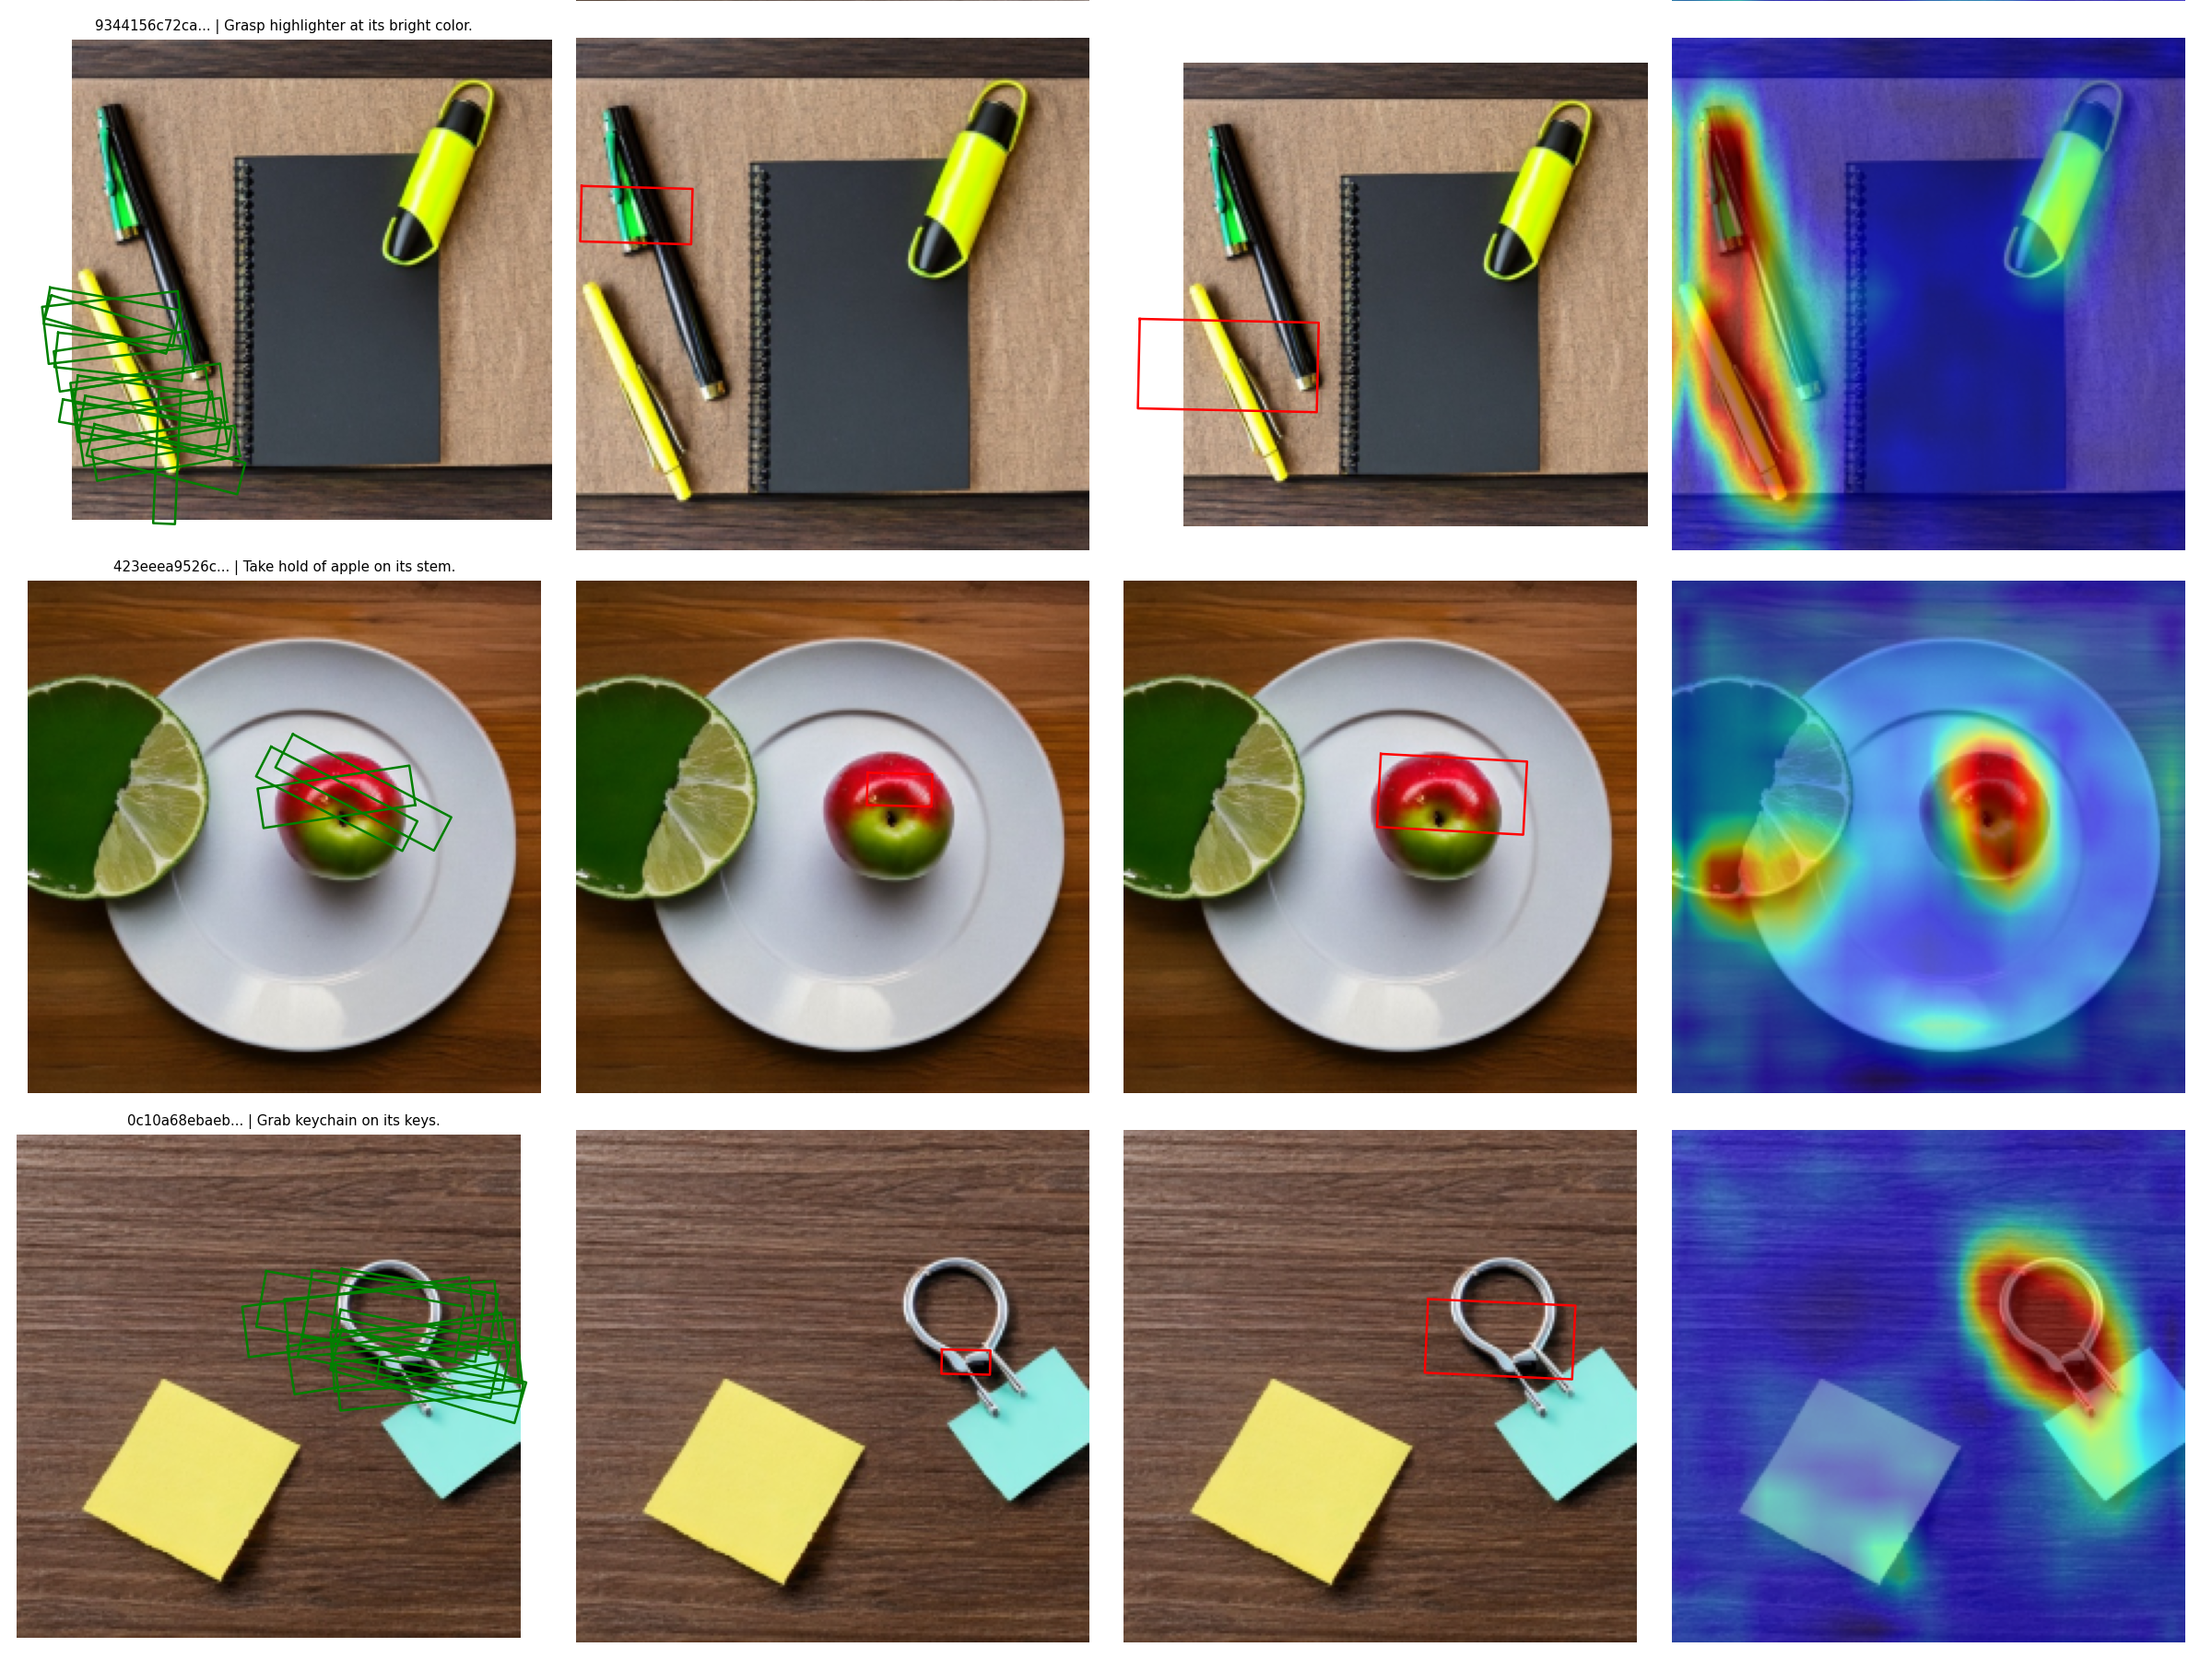
\includegraphics[width=0.98\linewidth]{figures/qualitative_paper.png}
\caption{Paired qualitative results: input, ground truth, LGDM prediction,
LSAR prediction, and LSAR affordance map.}
\label{fig:qual}
\end{figure}
